\documentclass[a4paper]{article}

%%% usepackage %%%
\usepackage{color}
\usepackage{graphicx}
\usepackage[inner=3cm, outer=3cm, top=3cm, bottom=3cm]{geometry}
\usepackage{xepersian}
\settextfont{Dubai}
\fontsize{30}{12}\selectfont



%%% newcommand %%%
\newcommand{\mynote}{\textbf {\large {\color{red} Note:  }}}
\newcommand{\myx}{\texttt{X}}
\newcommand{\true}{\texttt{T}}
\newcommand{\false}{\texttt{F}}
\newcommand{\emailone}{\texttt{abbas.yazdanmehr1@gmail.com}}
\newcommand{\fulltitle}[2]{\title{#1 \\ #2}}
\newcommand{\myinf}{
	\author{
عباس یزدان مهر
\\
99243077\\
 مهندسی کامپیوتر, دانشگاه شهید بهشتی
\\
\emailone
	}
}
\newcommand{\goodbye}{\begin{center}{\huge
پایان
}\end{center}}



\begin{document}

\fulltitle{
طراحی سیستم های دیجیتال
}{
تمرین اول
}

\myinf

\maketitle

\newpage


\section{}
\subsection{\begin{latin}$F = AC + BC + B $\end{latin}}


\subsection*{جدول درستی}
\begin{latin}
\begin{center}
\begin{tabular}{|c|c|c||c|}
\hline
A & B & C & F \\
\hline
\hline
0 & 0 & 0 & 0 \\
\hline
0 & 0 & 1 & 0 \\
\hline
0 & 1 & 0 & 1 \\
\hline
0 & 1 & 1 & 1 \\
\hline
1 & 0 & 0 & 0 \\
\hline
1 & 0 & 1 & 1 \\
\hline
1 & 1 & 0 & 1 \\
\hline
1 & 1 & 1 & 1 \\
\hline
\end{tabular}\end{center}
\end{latin}

\subsection*{جدول کارنو}
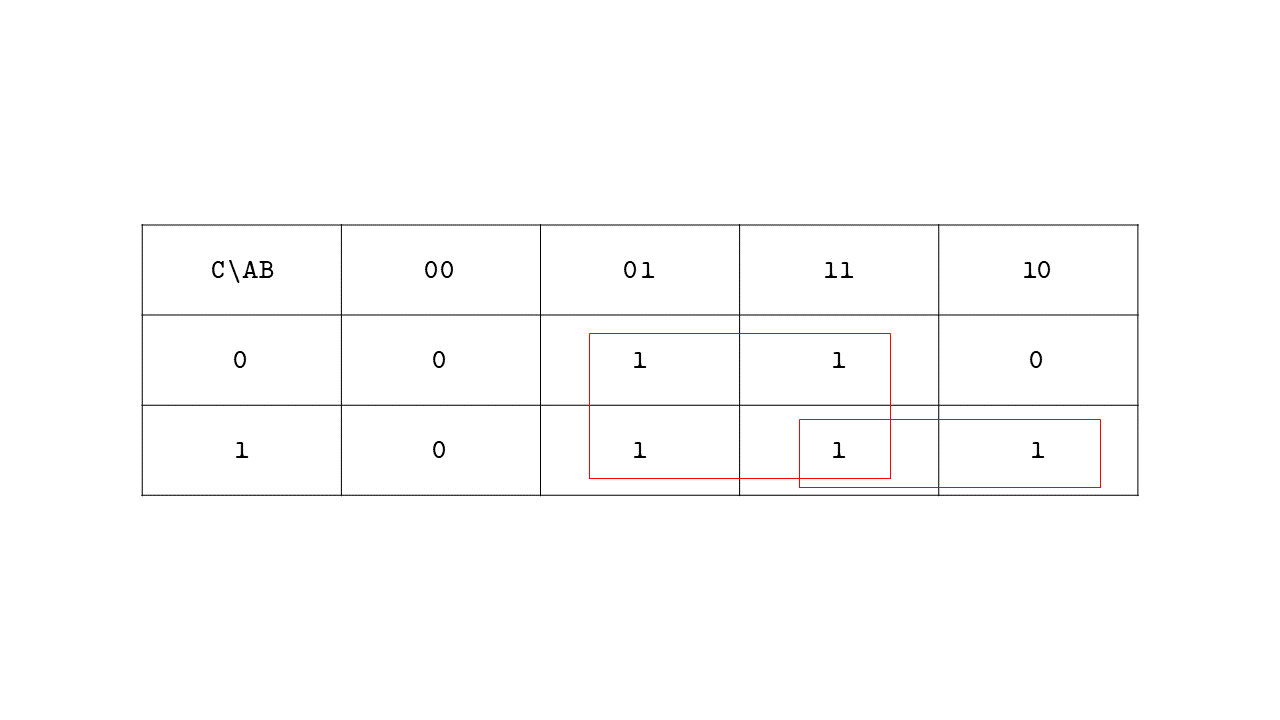
\includegraphics[width=10cm]{images/karno1_1.png}

\begin{latin}
$ \Longrightarrow SOP: F = B + AC $
\end{latin}

\subsection*{شماتیک}
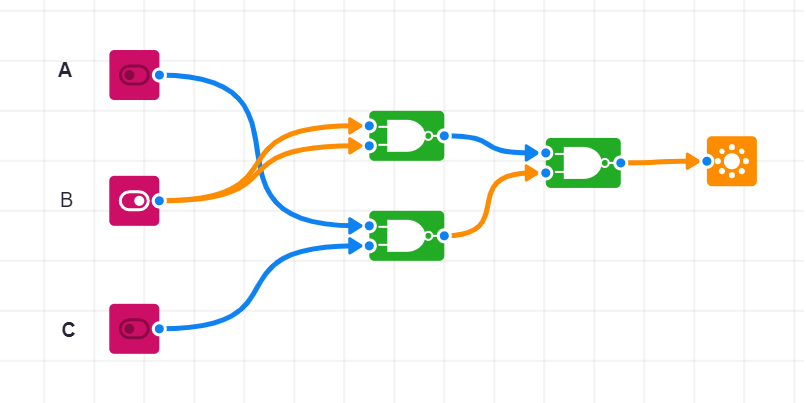
\includegraphics[width=10cm]{images/nand1_1.png}


\subsection{\begin{latin}$F(A, B, C, D) = \Sigma (0, 1, 2, 3, 4, 8, 9, 12) $\end{latin}}
\subsection*{جدول درستی}
\begin{latin}
\begin{center}
\begin{tabular}{|c|c|c|c||c|}
\hline
A & B & C & D & F \\
\hline
\hline
0 & 0 & 0 & 0 & 1 \\
\hline
0 & 0 & 0 & 1 & 1 \\
\hline
0 & 0 & 1 & 0 & 1 \\
\hline
0 & 0 & 1 & 1 & 1 \\
\hline
0 & 1 & 0 & 0 & 1 \\
\hline
0 & 1 & 0 & 1 & 0 \\
\hline
0 & 1 & 1 & 0 & 0 \\
\hline
0 & 1 & 1 & 1 & 0 \\
\hline
1 & 0 & 0 & 0 & 1 \\
\hline
1 & 0 & 0 & 1 & 1 \\
\hline
1 & 0 & 1 & 0 & 0 \\
\hline
1 & 0 & 1 & 1 & 0 \\
\hline
1 & 1 & 0 & 0 & 1 \\
\hline
1 & 1 & 0 & 1 & 0 \\
\hline
1 & 1 & 1 & 0 & 0 \\
\hline
1 & 1 & 1 & 1 & 0 \\
\hline
\end{tabular}
\end{center}
\end{latin}

\subsection*{جدول کارنو}
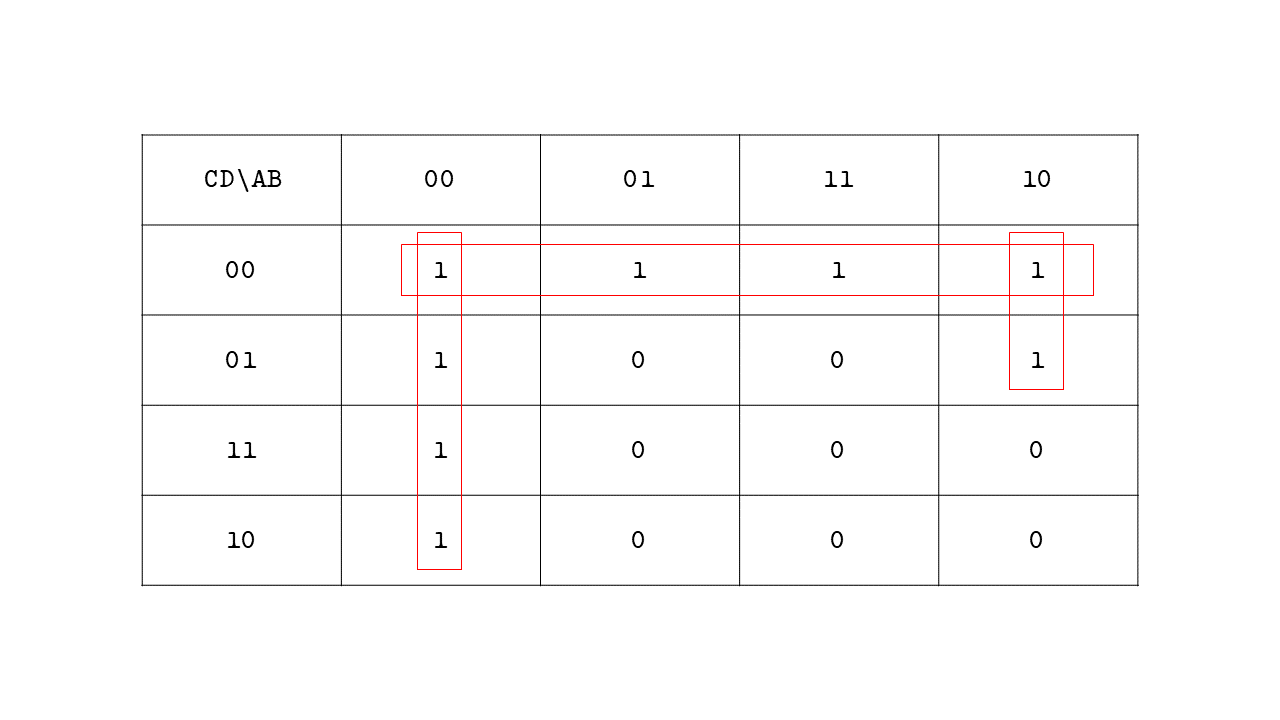
\includegraphics[width=10cm]{images/karno1_2.png}

\begin{latin}
$ \Longrightarrow SOP: F = \neg A \neg B + \neg C \neg D + \neg B \neg C $
\end{latin}

\subsection*{شماتیک}
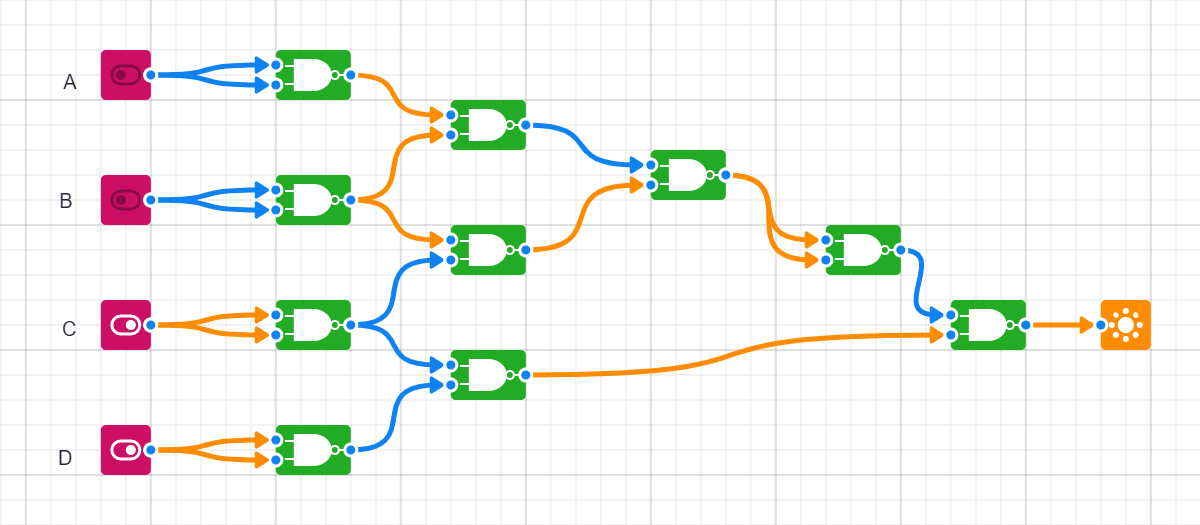
\includegraphics[width=10cm]{images/nand1_2.png}

\section{}
الف) سمت چپ تساوی را ساده می کنیم تا به سمت راست تساوی برسیم:
\\
\begin{latin} \noindent
					\mynote $ P + P'Q = P + Q $ \\
					\mynote $ P + P' = \true $ \\
					\mynote $ P(Q + R) = PQ + PR $ \\
					\mynote $ P + QR = (P + Q)(P + R) $ \\
 \end{latin}
\begin{tabular}{l l}
$ = A'BC + B'C'(A+A') + AB'C + AB $ & \\
$ = A'BC + B'C' + AB'C + AB $ &  \\
$ = B(A'C + A) + B'(C' + AC)$ & \\
$ = B(C + A) + B'(C' + A)$ & \\
$ = BC + AB + B'C' + AB'$ & \\
$ = BC + B'C' + A(B + B')$ & \\
$ = A + BC + B'C' $ & \\
\end{tabular}
\\[1cm]
ب) سمت چپ تساوی را ساده سازی می کنیم تا به سمت راست تساوی برسیم:
\\
\begin{latin} \mynote $ P + P'Q = P + Q $ \end{latin}
\begin{center}
\begin{tabular}{l l}
$ = A + A'(B + B'(C + C'D)) $ &  \\
$ = A + A'(B + B'(C + D)) $ & \\
$ = A + A'(B + (C + D)) $ & \\
$ = A + (B + (C + D)) $ & \\
$ = A + B + C + D $ & \\
\end{tabular}
\end{center}

\section{}

\begin{latin}
\begin{center}
\begin{tabular}{c|c|c||c|c}
A & B & C & carry & sum \\
\hline
\hline
0 & 0 & 0 & 0 & 0 \\
\hline
0 & 0 & 1 & 0 & 1 \\
\hline
0 & 1 & 0 & 0 & 1 \\
\hline
0 & 1 & 1 & 1 & 0 \\
\hline
1 & 0 & 0 & 0 & 1 \\
\hline
1 & 0 & 1 & 1 & 0 \\
\hline
1 & 1 & 0 & 1 & 0 \\
\hline
1 & 1 & 1 & 1 & 1 \\
\hline
\end{tabular}
\end{center}
\end{latin}

\begin{center}
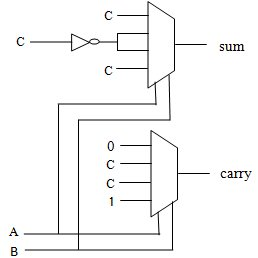
\includegraphics[width=5cm]{images/mux-sol.jpg}
\end{center}



\section{}
\begin{center}
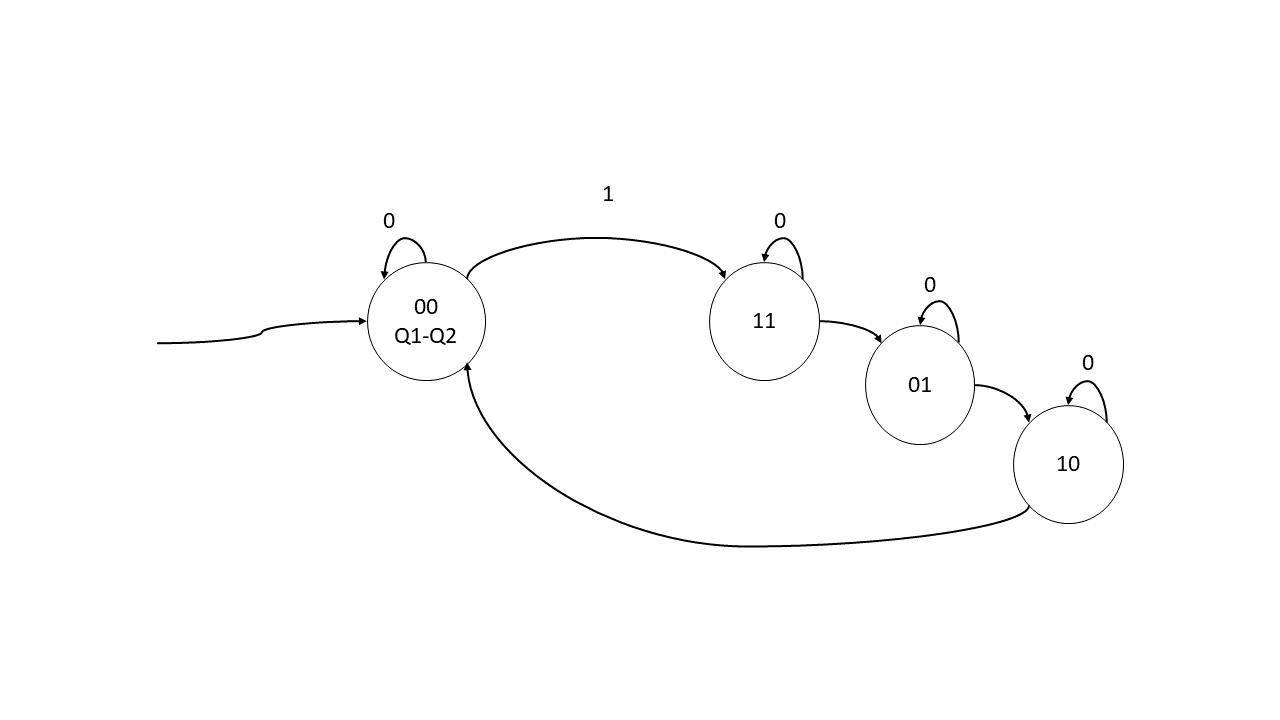
\includegraphics[width=10cm]{images/state-machine-2.png}
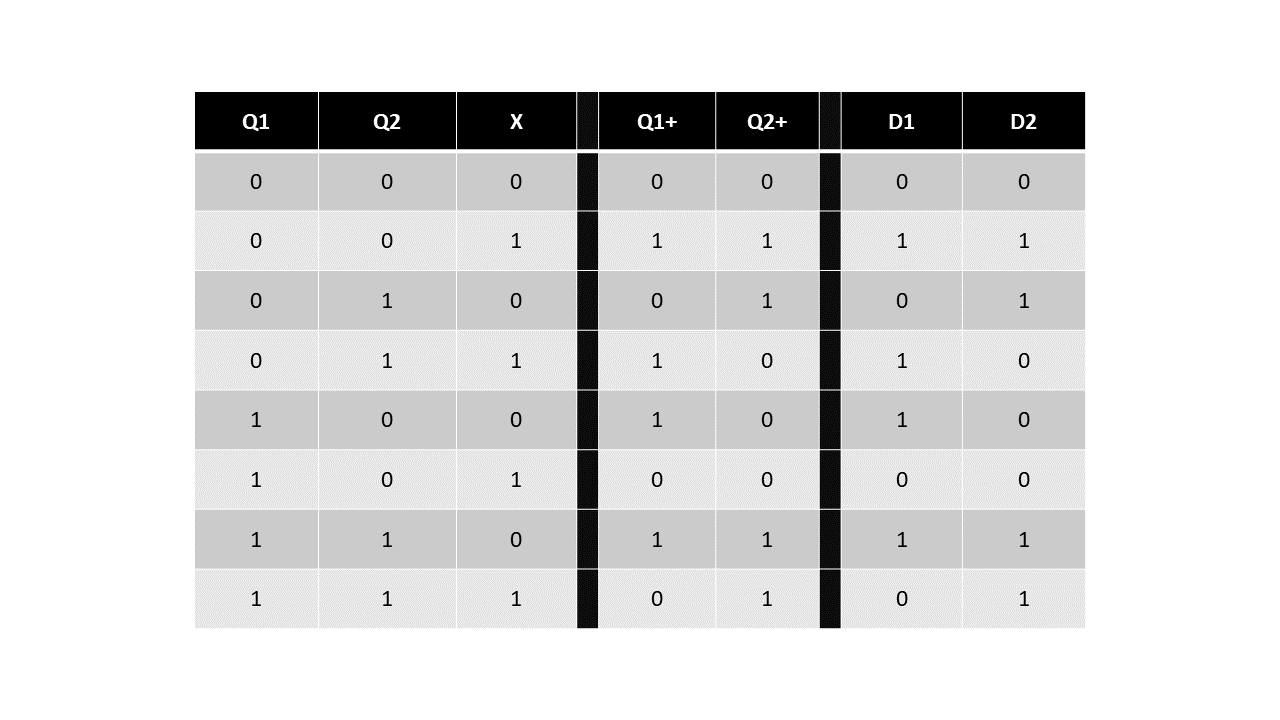
\includegraphics[width=10cm]{images/truth-table.png}
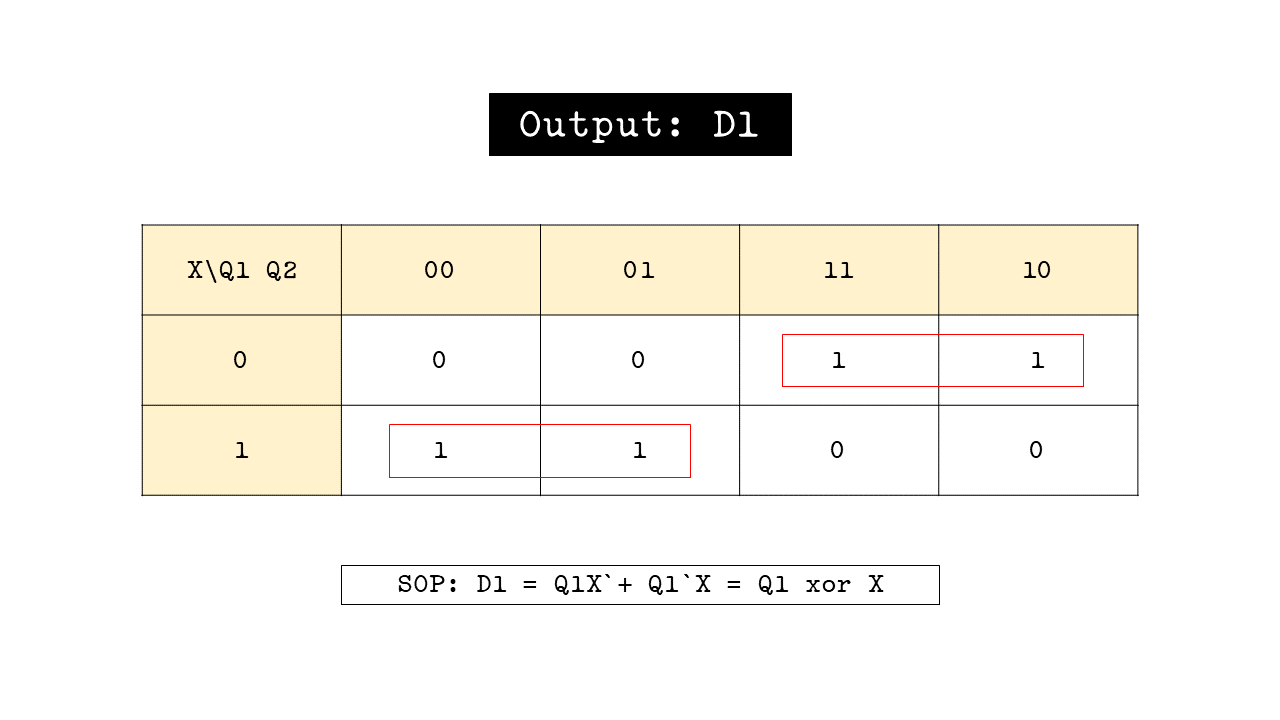
\includegraphics[width=10cm]{images/d1.png}
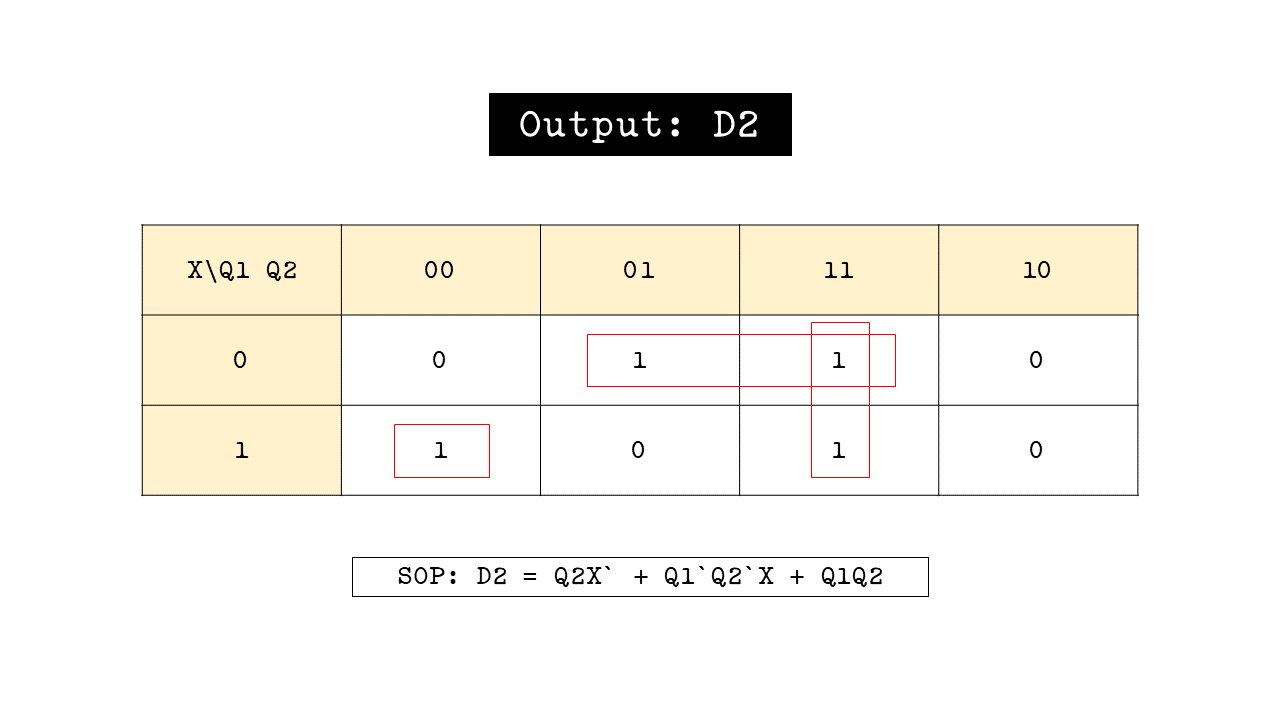
\includegraphics[width=10cm]{images/d2.png}
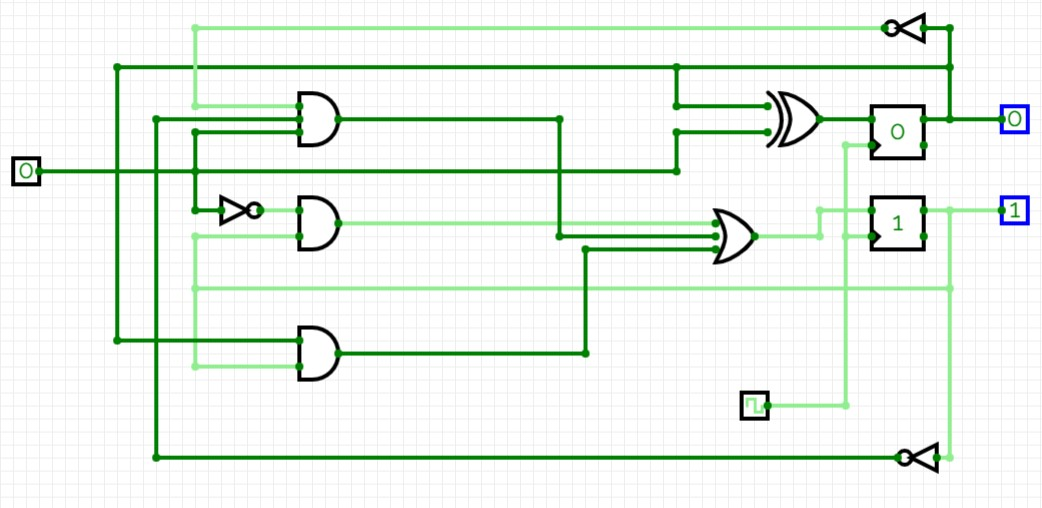
\includegraphics[width=10cm]{images/big-cir.jpg}
\end{center}

\section{}
\begin{displaymath}
99243077 \rightarrow 9 + 9 + 2 + 4 + 3 + 0 + 7 + 7 = 41 = 101001_{bin} \rightarrow A = 001
\end{displaymath}

\subsection*{ماشین حالت:}
\begin{center}
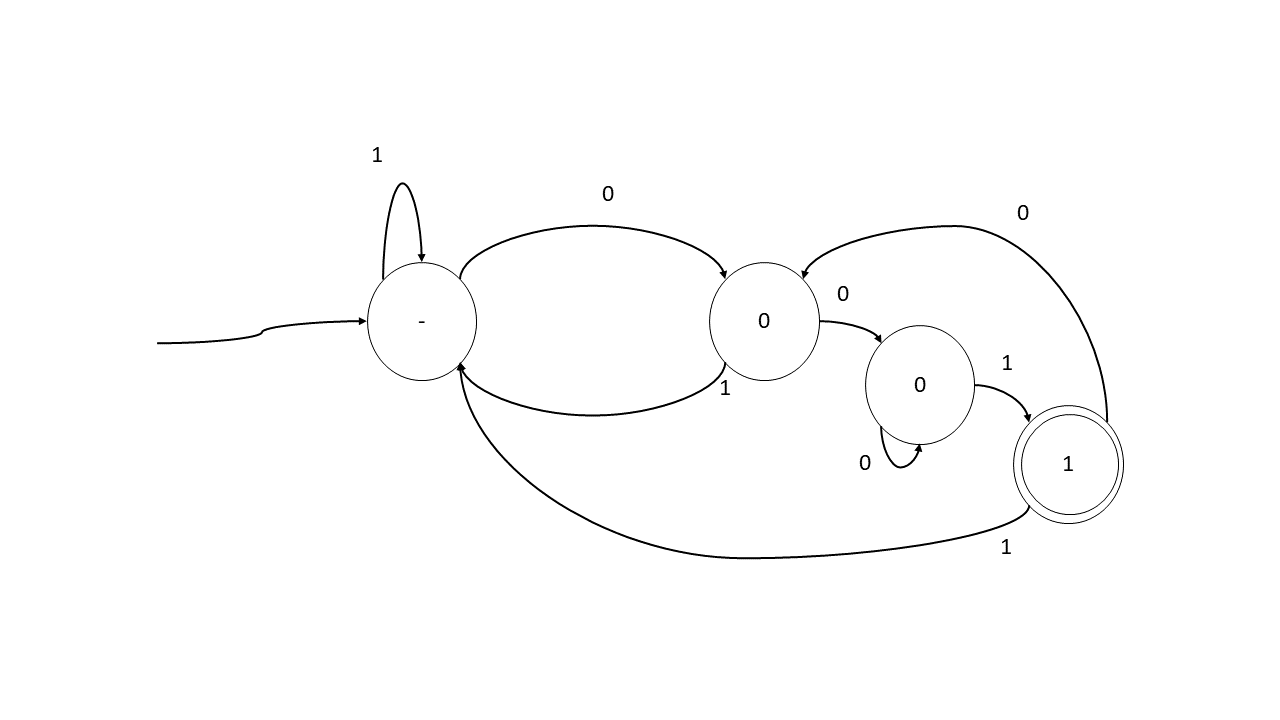
\includegraphics[width=10cm]{images/state-machine.png}
\end{center}

\newpage
\goodbye
\end{document}
